\href{https://github.com/mfclabber/itmo-cv-labs/tree/main/lab6}{Исходный код на GitHub}. 

Для удобства отладки и сборки используется средство автоматизации сборки ПО CMake:
\begin{lstlisting}[style=cpp_white, caption={CMakeLists.txt для сборки проекта}]
cmake_minimum_required(VERSION 2.8)

project( CV_LW6 )
find_package( OpenCV REQUIRED )

include_directories( ${OpenCV_INCLUDE_DIRS} )
add_executable( ${PROJECT_NAME}  src/lab6.cpp )

target_link_libraries( ${PROJECT_NAME} ${OpenCV_LIBS} )
\end{lstlisting}

\section{Базовые морфологические операции}

Морфологические операции над изображениями зачастую используются в качестве препроцессинга для работы с медицинскими снимками.
Возьмем один снимок из датасета \href{https://www.kaggle.com/datasets/trainingdatapro/multiple-sclerosis-dataset}{Brain MRI} и применим к нему морфологические операции для удаления ненужных областей снимка.

\begin{figure}[H]
    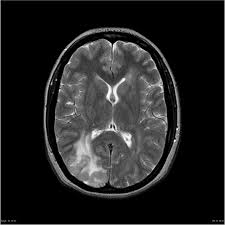
\includegraphics[width=\textwidth]{../source/1.png}
    \caption{Исходное изображение}
\end{figure}

\begin{lstlisting}[style=cpp_white, caption={Исходный код для отделения мозга от}]
cv::Mat image;
image = cv::imread(path + "/source/1.png", 0);

cv::Mat labelImage(image.size(), CV_32S);

cv::Mat new_image = cv::Mat::zeros(image.rows, image.cols, image.type());

int morph_size = 2; 
cv::Mat kernel = getStructuringElement(cv::MORPH_RECT, 
                                        cv::Size(1 * morph_size + 1, 
                                                1 * morph_size + 1), 
                                        cv::Point(morph_size, 
                                                    morph_size)); 

cv::erode(image, new_image, kernel, cv::Point(-1, -1), 1); //, cv::BORDER_CONSTANT, cv::morphologyDefaultBorderValue());

int n_labels = connectedComponents(new_image, labelImage, 4);
std::unordered_map<int, int> labels_map;

for(int i = 0; i < image.rows-1; ++i){
    for(int j = 0; j < image.cols-1; ++j){
        ++labels_map[labelImage.at<int>(i, j)];
    }
}

labels_map.erase(0);

int k = (*std::max_element(labels_map.begin(), labels_map.end(), [](auto a, auto b){return a.second < b.second;})).first;

for(int i = 0; i < image.rows-1; ++i){
    for(int j = 0; j < image.cols-1; ++j){
        if(labelImage.at<int>(i, j) == k)
            new_image.at<uchar>(i, j) = new_image.at<uchar>(i, j);
        else
            new_image.at<uchar>(i, j) = 0;
    }
}

cv::morphologyEx(new_image, new_image, 
                    cv::MORPH_DILATE, kernel, 
                    cv::Point(-1, -1), 2); 

cv::morphologyEx(new_image, new_image, 
                    cv::MORPH_GRADIENT, kernel, 
                    cv::Point(-1, -1), 2); 

cv::imwrite(path + "/outputs/1_gradient.png", new_image);
cv::imshow("image", new_image);
cv::waitKey();
\end{lstlisting}

Как удалось столь успешно получить требуемый результат? Сначала применили эрозию для более точного отделения черепа от мозга (между ними есть очень слабая корреляция, что не давало прмиенить connectedComponents), 
дальше составили матрицы смежных компонент и вычислили преобладающую компоненту (она же мозг), предварительно вырезав компоненту фона. Применив дилатацию, мы частично убираем эффект эрозии и получаем маску мозга, которую можно наложить на исходное изображение и получить точный снимок мозга.

\begin{figure}[H]
    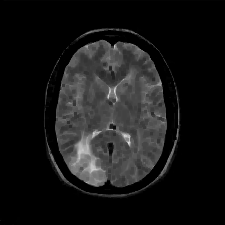
\includegraphics[width=\textwidth]{../outputs/1_erode.png}
    \caption{Результат применения эрозии}
\end{figure}

\begin{figure}[H]
    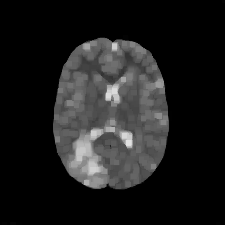
\includegraphics[width=\textwidth]{../outputs/1_erode_dilate.png}
    \caption{Результат применения эрозии + удаления области черепа + дилатации}
\end{figure}

Посмотрим на морфлогический градиент, который покаывает разницу дилатации и эрозии.

\begin{figure}[H]
    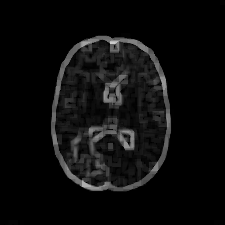
\includegraphics[width=\textwidth]{../outputs/1_gradient.png}
    \caption{Морфологический градиент области мозга}
\end{figure}

\begin{figure}[H]
    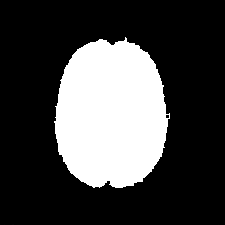
\includegraphics[width=\textwidth]{../outputs/1_mask.png}
    \caption{Бинарная маска мозга}
\end{figure}

\begin{figure}[H]
    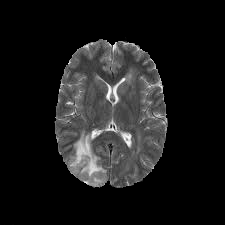
\includegraphics[width=\textwidth]{../outputs/1_res.png}
    \caption{Результирующее изображение}
\end{figure}




\section{Разделение объектов}

Выберем произвольное изображение, содержащее перекрывающиеся объекты. С помощью операций бинарной морфологии для разделим объекты. Выделим их контуры.

\begin{figure}[H]
    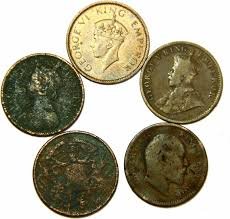
\includegraphics[width=\textwidth]{../source/3.png}
    \caption{Исходное изображение}
\end{figure}

\begin{lstlisting}[style=cpp_white, caption={Исходный код для разделения и выделения контуров}]
cv::Mat image, new_image, BW2;
image = cv::imread(path + "/source/3.png", 0);

cv::threshold(image, new_image, 160, 255, cv::THRESH_BINARY_INV);

cv::Mat kernel = cv::getStructuringElement(cv::MORPH_ELLIPSE, cv::Size(5, 5));

cv::morphologyEx(new_image, BW2, cv::MORPH_ERODE, kernel, cv::Point(-1, -1), 14, cv::BORDER_CONSTANT, cv::Scalar(0));

cv::Mat D, S, C;
cv::Mat T = cv::Mat::zeros(new_image.rows, new_image.cols, new_image.type());

int pix_num = new_image.rows * new_image.cols;

while(cv::countNonZero(BW2) < pix_num){
    cv::morphologyEx(BW2, D, cv::MORPH_DILATE, kernel, cv::Point(-1, -1), 1, cv::BORDER_CONSTANT, cv::Scalar(0));
    cv::morphologyEx(D, C, cv::MORPH_CLOSE, kernel, cv::Point(-1, -1), 1, cv::BORDER_CONSTANT, cv::Scalar(0));
    S = C - D;
    cv::bitwise_or(S, T, T);
    BW2 = D;
}

cv::morphologyEx(T, T, cv::MORPH_CLOSE, kernel, cv::Point(-1, -1), 1, cv::BORDER_CONSTANT, cv::Scalar(255));
cv::bitwise_and(T,  new_image, new_image);
std::cout << 'a';
cv::imshow("image", new_image);
cv::waitKey();
\end{lstlisting}

\begin{figure}[H]
    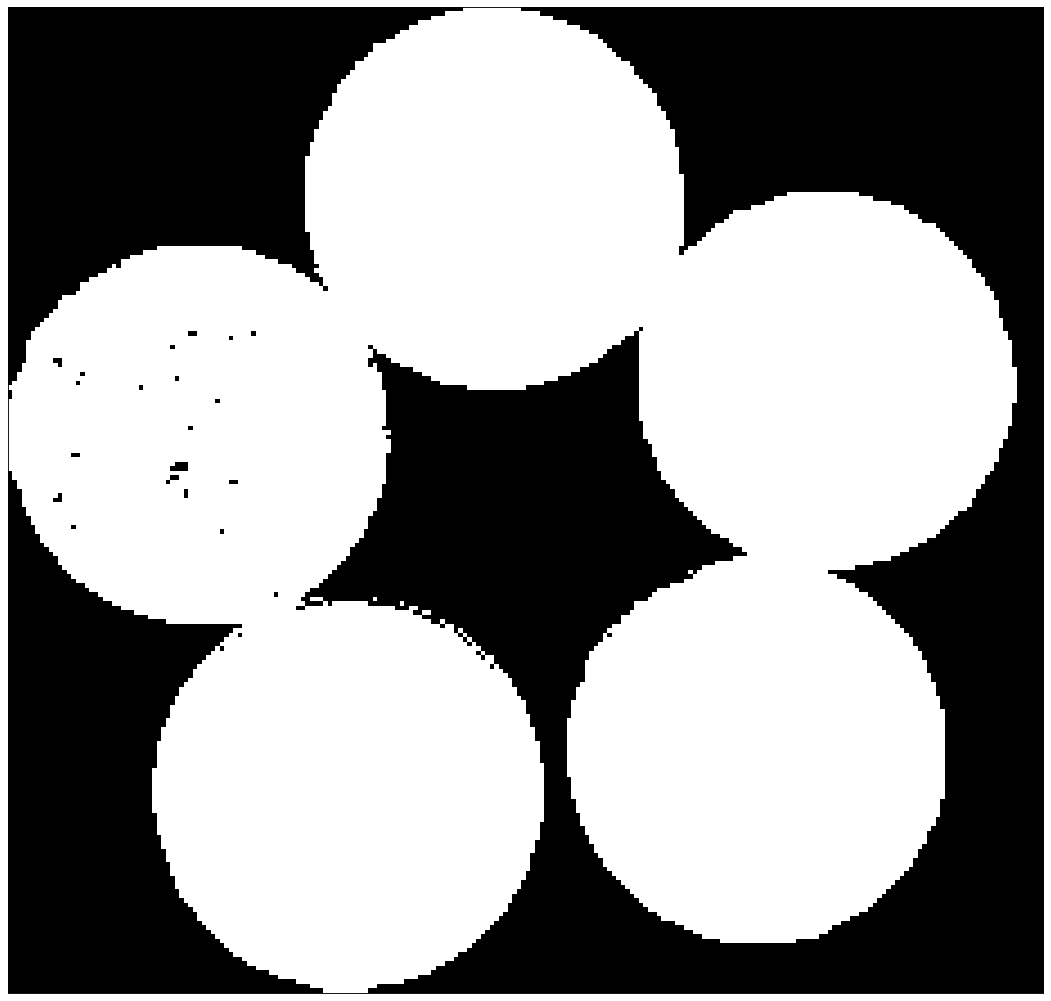
\includegraphics[width=\textwidth]{../outputs/2_mask.png}
    \caption{Бинаризованное изображение}
\end{figure}

\begin{figure}[H]
    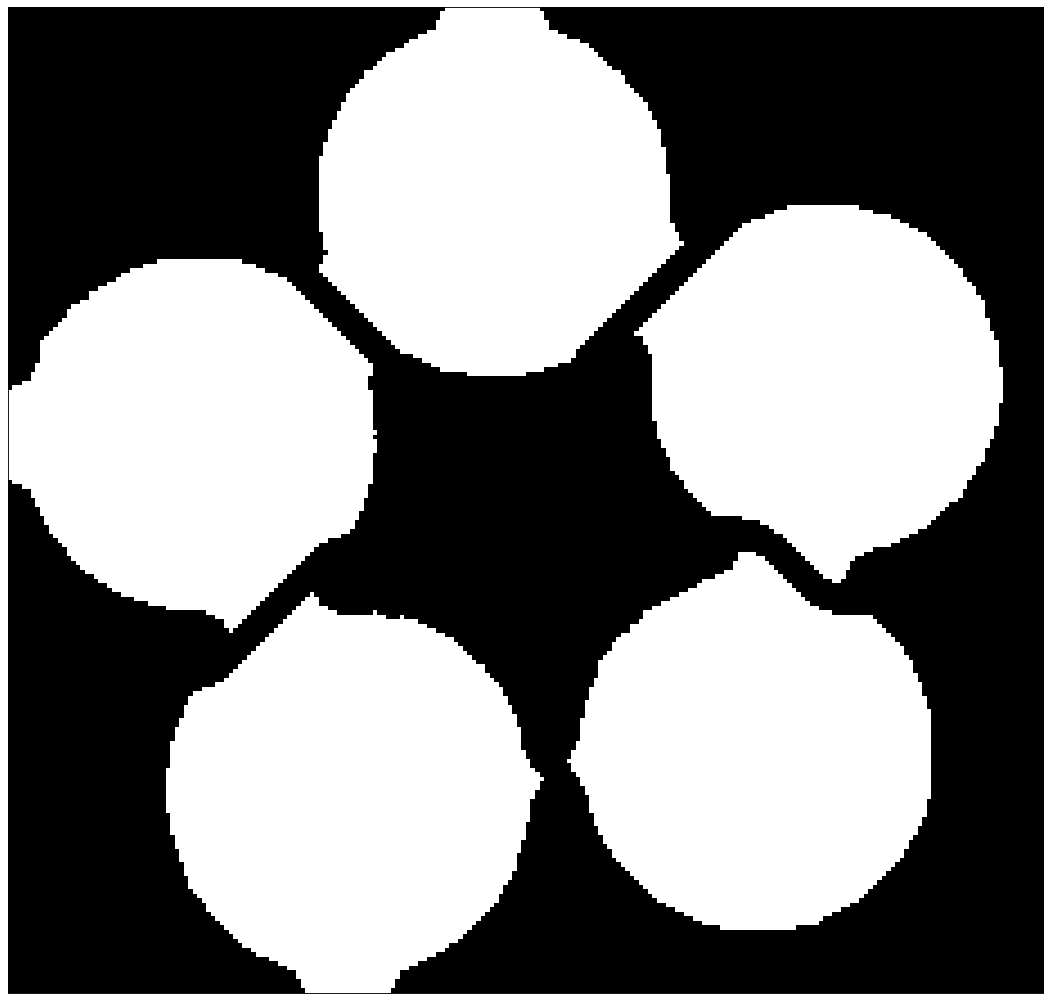
\includegraphics[width=\textwidth]{../outputs/2_diff.png}
    \caption{Бинарная маска после разделения объектов}
\end{figure}

\begin{figure}[H]
    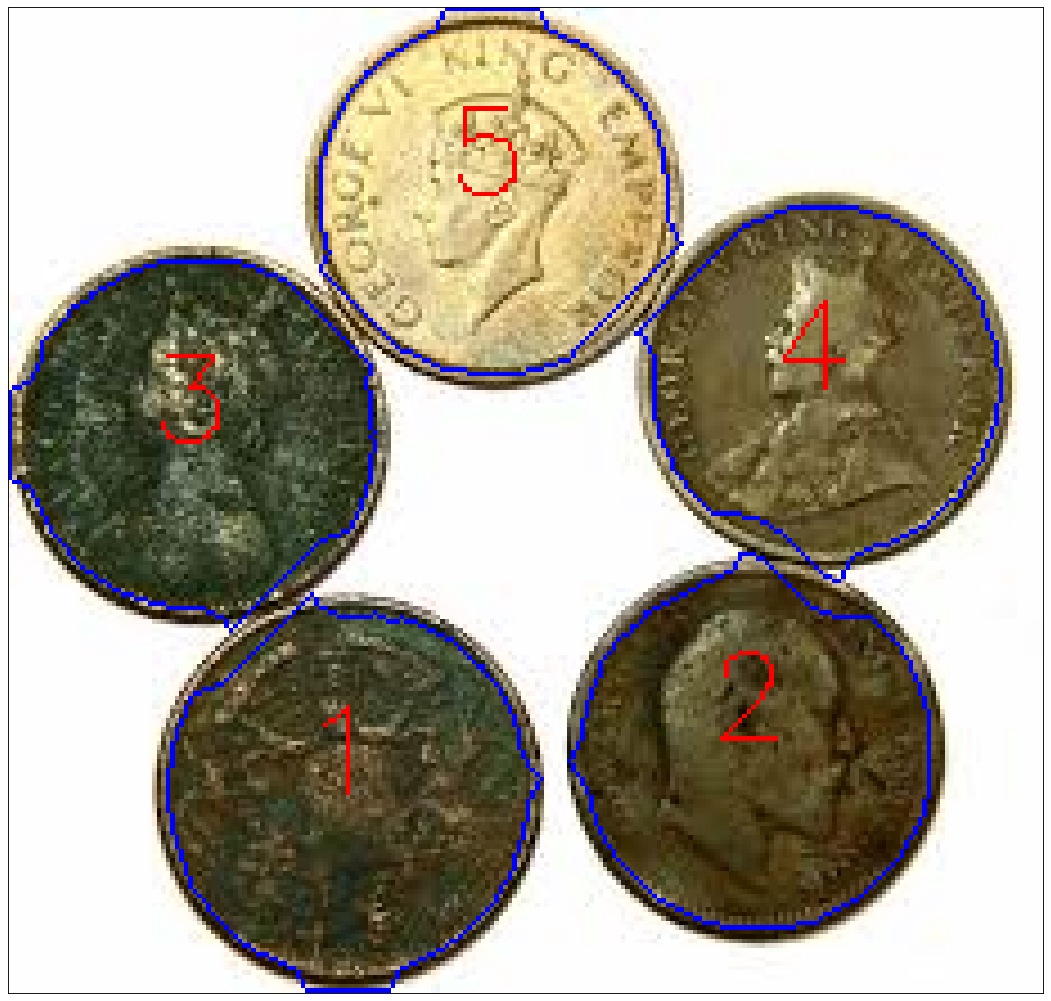
\includegraphics[width=\textwidth]{../outputs/2_edge.png}
    \caption{Результирующее изображение с выделенными контурами и подсчитанными монетками}
\end{figure}


\section{Сегментация изображения по водоразделам}

Выберем произвольное изображение, содержащее небольшое число локальных минимумов. Выполним сегментацию изображения по водоразделам.

\begin{figure}[H]
    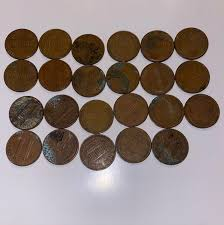
\includegraphics[width=\textwidth]{../source/2.png}
    \caption{Исходное изображение}
\end{figure}

\begin{lstlisting}[style=cpp_white, caption={Исходный код для сегментации изображения по водоразделам}]
cv::Mat image, image_gray, image_bw;
image = cv::imread(path + "/source/2.png", 1);

cv::cvtColor(image, image_gray, cv::COLOR_BGR2GRAY);
cv::threshold(image_gray, image_bw, 0, 250, cv::THRESH_BINARY + cv::THRESH_OTSU);

bwareaopen(image_bw, image_bw, 20, 8);
cv::Mat B = cv::getStructuringElement(cv::MORPH_ELLIPSE, cv::Size(5, 5));

cv::morphologyEx(image_bw, image_bw, cv::MORPH_CLOSE, B);


cv::Mat image_fg;
double image_fg_min, image_fg_max;
cv::distanceTransform(image_bw, image_fg, cv::DIST_L2, 5);

cv::minMaxLoc(image_fg, &image_fg_min, &image_fg_max);
cv::threshold(image_fg, image_fg, 0.7 * image_fg_max, 255, 0);
image_fg.convertTo(image_fg, CV_8U, 255.0 / image_fg_max);

cv::imshow("image", image_fg);
cv::waitKey();
cv::Mat markers;

int num = cv::connectedComponents(image_fg, markers);

cv::Mat image_bg = cv::Mat::zeros(image_bw.rows, image_bw.cols, image_bw.type());

cv::Mat markers_bg = markers.clone();
cv::watershed(image, markers_bg);

image_bg.setTo(cv::Scalar(255), markers_bg == -1);

cv::Mat image_unk;

cv::bitwise_not(image_bg, image_unk);
cv::subtract(image_unk, image_fg, image_unk);

markers += 1;
markers.setTo(cv::Scalar(0), image_unk == 255);

cv::watershed(image, markers);

cv::Mat markers_jet;
markers.convertTo(markers_jet, CV_8U, 255.0 / (num + 1));

cv::applyColorMap(markers_jet, markers_jet, cv::COLORMAP_JET);

image.setTo(cv::Scalar(255, 0, 0), markers == -1);
cv::imwrite(path + "/outputs/3_filtr_reverse.png", image_fg);
cv::imshow("image", image_bg);
cv::waitKey();
\end{lstlisting}

\begin{figure}[H]
    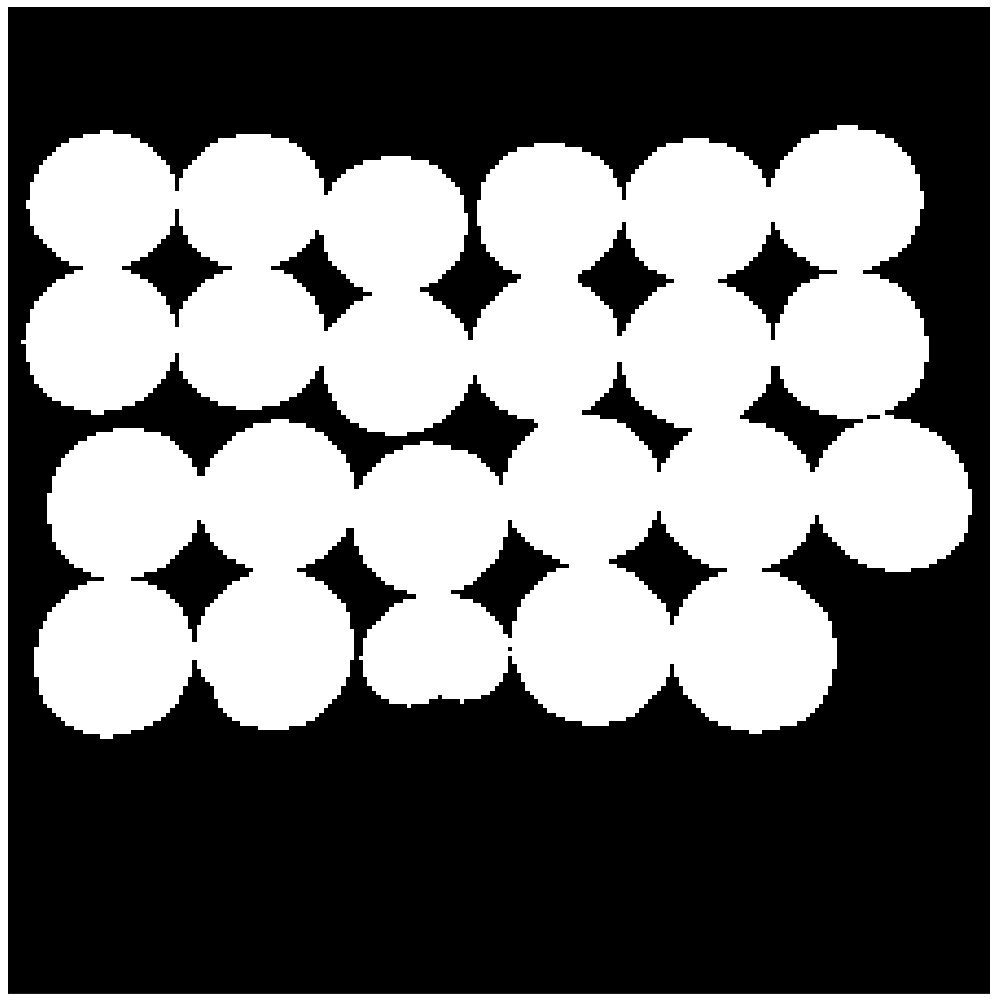
\includegraphics[width=\textwidth]{../outputs/3_filtr.png}
    \caption{Бинаризованное изображение}
\end{figure}

\begin{figure}[H]
    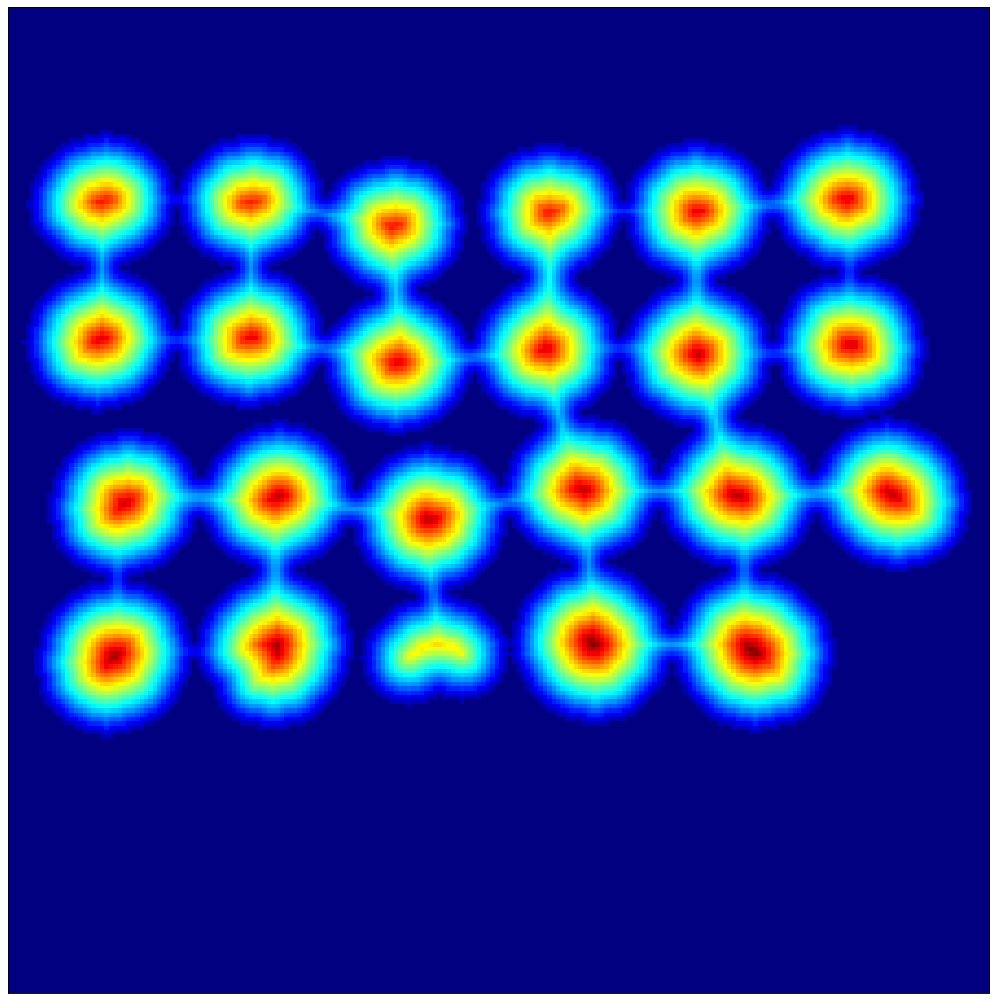
\includegraphics[width=\textwidth]{../outputs/3_map_of_heights.png}
    \caption{Карта интенсивностей пикселей изображения}
\end{figure}

\begin{figure}[H]
    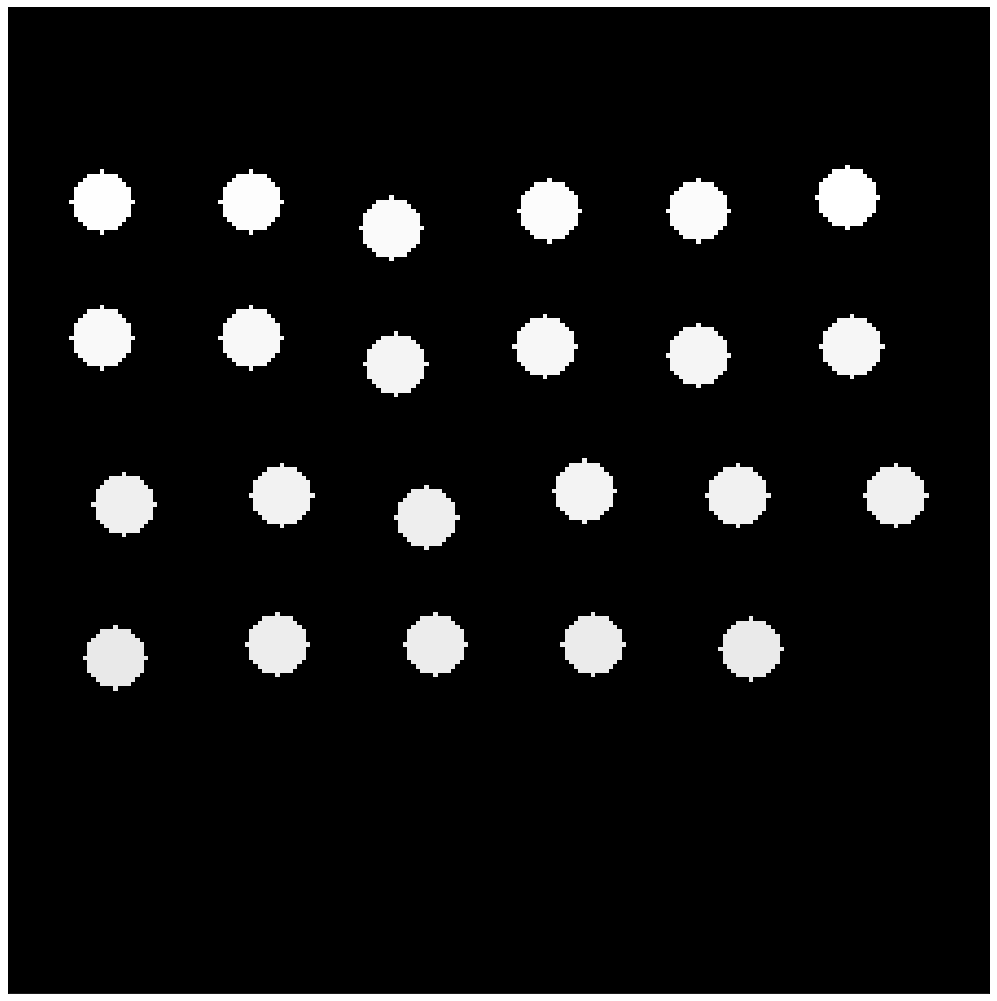
\includegraphics[width=\textwidth]{../outputs/3_map_local_min.png}
    \caption{Объединение маркеров переднего и заднего плана}
\end{figure}

\begin{figure}[H]
    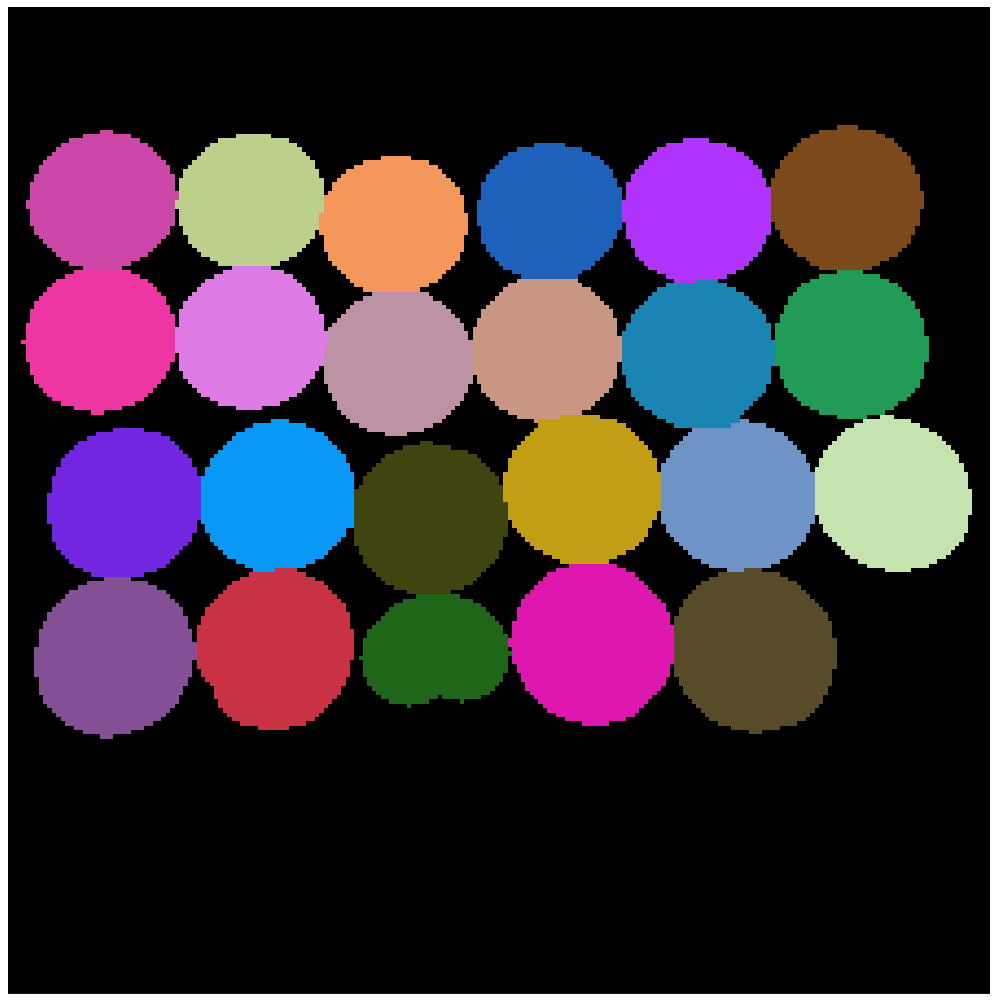
\includegraphics[width=\textwidth]{../outputs/3_segmentation.png}
    \caption{Результат сегментации}
\end{figure}

\begin{figure}[H]
    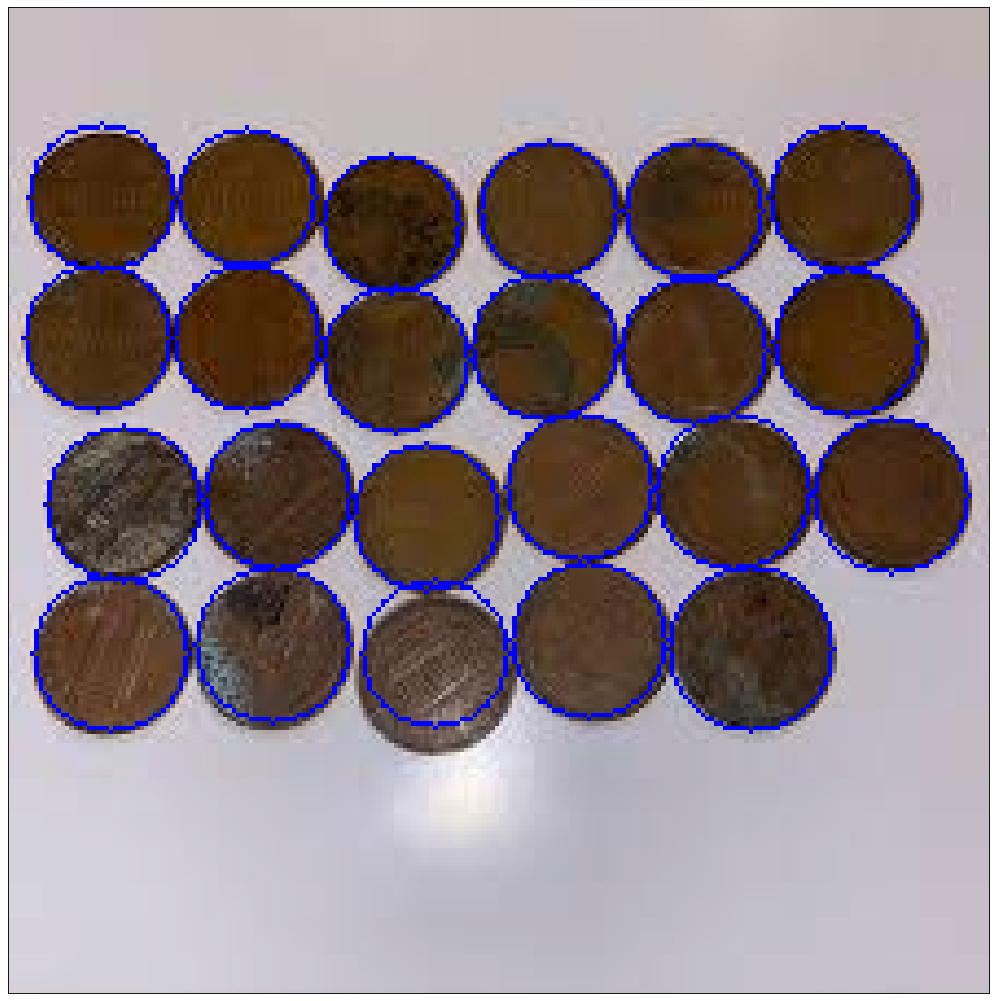
\includegraphics[width=\textwidth]{../outputs/3_result.png}
    \caption{Выделение контуров}
\end{figure}


\section{Ответы на вопросы}

\newcounter{question}
\setcounter{question}{0}

\newcommand{\question}[1]{\item[Q\refstepcounter{question}\thequestion.] #1}
\newcommand{\answer}[1]{\item[A\thequestion.] #1}

\begin{itemize}

\question{Включает ли результат открытия в себя результат закрытия?}
\answer{
    В математической морфологии результат открытия не включает в себя результат закрытия. Открытие и закрытие - это две разные операции, которые могут применяться к изображениям для достижения различных целей.
    
    Открытие - это операция, при которой изображение сначала эрозируется (обычно с использованием структурного элемента) и затем расширяется. Открытие полезно для удаления шума или размытия объектов на изображении без значительного изменения размера объектов.
    
    Закрытие - это операция, при которой изображение сначала расширяется, а затем эрозируется. Закрытие полезно для заполнения маленьких дырок в объектах или соединения близко расположенных объектов.
    
    Таким образом, результат открытия и закрытия в математической морфологии обычно не эквивалентны.}

\question{Какой морфологический фильтр необходимо применить, чтобы убрать у объекта выступы?}
\answer{
Для удаления выступов с объекта на изображении можно использовать операцию "открытия" в математической морфологии.

Открытие состоит из двух этапов: сначала применяется операция "эрозии" для удаления маленьких деталей или шума, а затем операция "расширения" для восстановления оставшихся объектов до исходного размера.

Применение операции открытия поможет удалить выступы с объекта, сохраняя его основную форму и структуру.
}

\question{Каким образом с помощью морфологических операций можно
найти контур объекта?}
\answer{
    Для нахождения контура объекта с помощью морфологических операций можно использовать операцию "разности" или "градиента".

    Операция разности: Для этого сначала нужно применить операцию "закрытия" к изображению для заполнения мелких дырок в объекте и сглаживания его границ. Затем применяется операция "разности" между исходным изображением и результатом закрытия. Это позволит выделить контур объекта.
    Операция градиента: Эта операция выполняет разность между расширенным и эрозированным изображением. При этом выделяются грани объектов. Результатом будет изображение, на котором выделены контуры объектов.
    Использование одной из этих операций поможет найти контур объекта на изображении.}


\question{Что такое морфология?}
\answer{
    Морфология в контексте обработки изображений - это область обработки изображений, которая изучает структуру, форму и связи объектов на изображениях. Она основана на математических концепциях и операциях, а также вдохновлена идеями из математической морфологии, которая изначально занималась изучением форм и структур в естественных объектах.

    Морфологические операции включают в себя такие действия, как эрозия, расширение, открытие, закрытие, размыкание, замыкание и др. Они используются для изменения формы объектов на изображениях, удаления шума, выделения контуров объектов, заполнения дырок и различных других преобразований, которые помогают улучшить качество и анализ изображений..}

\end{itemize}

